\chapter{Abstract}
In this report, we introduce an exciting topic of Image Segmentation, discuss its role in imaging systems and articulate different approaches to segmentation beyond global thresholding. We briefly elaborate on different techniques towards segmentation followed by testing those approaches on a set of given inclass images and additional images chosen by our team which are diverse and as challenging as the inclass images. We strive not to compose a subjective implementation of algorithm which is not reusable on diverse set of segmentation tasks. Finally, we showcase the results of running those algorithm and conclude on evaluating segmentation methods.

\chapter{Introduction \& Background}
Image Segmentation is an interesting, important and active area of research and development. It has serious applications in medicine for e.g screening a human brain to detect an abnormality in early stages. The objective of segmentation is to divide an image into meaning regions. In other words, the task is to group pixels together based on certain characteristic for e.g color, shape, size, etc, such is a problem of segmentation. Human beings perceive image as a whole. For us, inferring information behind that image is a natural and intuitive task. On other hand, for machines, image is a matrix composed of numbers with varying intensities and therefore a machine tasked with segmentation is a difficult problem, mainly because of ambiguity in data. In this report, we  describe basic segmentation techniques which are based on \textbf{intensity discontinuity} useful for edge detection and also \textbf{similarity of intensity values}.
\begin{figure}[h]
  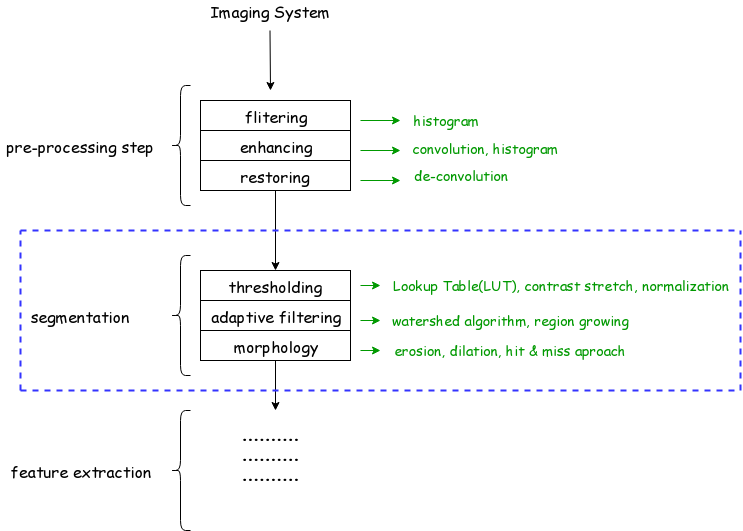
\includegraphics[width=15cm,height=10cm,keepaspectratio]{img/role_of_img_seg_diagram.png}
  \caption{The role of Image Segmentation as a pre-requisite step in feature extraction}
\end{figure}
The above figure describes a typical imaging system which incorporates Image Segmentation component in its pipeline. It receives input feed as a pre-processed image, performs segmentation with ultimate goal as classification, image compression, restoring image or simply monitoring task. In this case, the next layer is feature extraction which makes it evident that system is trying to solve classification problem. As you can see, in similar way, segmentation can be used as necessary addon based on overall purpose of the application.
%%% Local Variables:
%%% mode: latex
%%% TeX-master: "report"
%%% End:
